\documentclass[../../../../main.tex]{subfiles}
\begin{document}

\begin{flushright}
\footnotesize\textit{【自動文字起こし・要確認】}
\end{flushright}

\noindent
[\textbf{解}] $OX$ を $x$ 軸、$O$ を原点とする右のような座標を考え、$OY$ の方向ベクトル $\begin{pmatrix} \cos\theta \\ \sin\theta \end{pmatrix}$ とおく ($0 < \theta < \pi$)。又点 $A(\alpha, \beta)$ とおく。\\
題意から $P_1(t_1, 0)$, $Q_1(t_1\cos\theta, t_1\sin\theta)$, $P_2(t_2, 0)$, $Q_2(t_2\cos\theta, t_2\sin\theta)$ ($0 < t_1 < t_2$) とおける。$P_1 Q_1 \perp OA$ 又は $P_2 Q_2 \perp OA$ の時、$OP_1 = OQ_1$, $OP_2 = OQ_2$ から、$A$ は $\angle XOY$ の2等分線上にあるから、以下 $\angle OAP_1 \ne \pi/2$, $\angle OAP_2 \ne \pi/2$ とする。$\dots *$

\begin{center}
\begin{tikzpicture}[scale=1.2, >=stealth]
  \draw[->] (0,0) -- (3.5,0) node[right] {$x$};
  \draw[->] (0,0) -- (2.0,3.0) node[above right] {$Y$};
  \node[below left] at (0,0) {$O$};

  \coordinate (A) at (2.2, 1.8);
  \fill (A) circle (1.5pt) node[right] {$A$};

  \coordinate (P) at (1.2, 0);
  \coordinate (Q) at (0.8, 1.2);
  \draw[thick] (P) -- (Q);

  \draw[dashed] (A) -- (P);
  \draw[dashed] (A) -- (Q);

  \draw (0.5, 0) arc (0:56:0.5);
  \node at (0.7, 0.3) {$\theta$};
\end{tikzpicture}
\end{center}

\begin{align*}
\tan \angle OAP_1 &= \tan \angle OAQ_1 \\
\tan \angle OAP_2 &= \tan \angle OAQ_2
\end{align*}
ところで、右図の3点 $P, Q, R$ に対し
\[
\tan \theta = \frac{\sin\theta}{\cos\theta} = \frac{\overline{PQ} \cdot \overline{PR} \sin\theta}{\overline{PQ} \cdot \overline{PR} \cos\theta} = \frac{2 (\triangle PQR \text{の面積})}{\vec{PQ} \cdot \vec{PR}}
\]

\begin{center}
\begin{tikzpicture}[scale=1.2, >=stealth]
  \coordinate (P) at (0,0);
  \coordinate (Q) at (2.5, 1.2);
  \coordinate (R) at (2.0, -0.8);

  \draw[thick] (Q) -- (P) -- (R);
  \node[left] at (P) {$P$};
  \node[above right] at (Q) {$Q$};
  \node[below right] at (R) {$R$};

  \draw (0.6, 0.29) arc (25.6:-21.8:0.6);
  \node at (0.9, 0.05) {$\theta$};
\end{tikzpicture}
\end{center}

\noindent
だから $t_1, t_2$ は方程式
\begin{equation}
\frac{|\beta(t-\alpha) + \alpha\beta|}{-\alpha(t-\alpha) + \beta^2} = \frac{|\beta(t\cos\theta-\alpha) - \alpha(t\sin\theta-\beta)|}{-\alpha(t\cos\theta-\alpha) - \beta(t\sin\theta-\beta)} \dots \text{①}
\end{equation}
の2異実数解（ただし $C = \cos\theta, S = \sin\theta$ ときて、$\begin{pmatrix} \alpha \\ \beta \end{pmatrix} = r \begin{pmatrix} \cos\varphi \\ \sin\varphi \end{pmatrix}$ ($0 < r, 0 < \varphi < \theta$) とおいて、①に代入すると
\[
\frac{|r\sin\varphi \cdot t|}{-r\cos\varphi \cdot t + r^2} = \frac{|r(\sin\varphi \cdot C - \cos\varphi \cdot S) t|}{-r(\cos\varphi \cdot C + \sin\varphi \cdot S) t + r^2}
\]
$t > 0, \sin\varphi > 0, t > 0, \sin(\theta-\varphi) > 0$ から
\[
\frac{\sin\varphi}{-\cos\varphi \cdot t + r} = \frac{\sin(\theta-\varphi)}{-\cos(\theta-\varphi) \cdot t + r}
\]
\[
\left(\sin\varphi \cos(\theta-\varphi) - \sin(\theta-\varphi)\cos\varphi\right) t + r\left(\sin\varphi - \sin(\theta-\varphi)\right) = 0
\]
\begin{equation}
\sin(2\varphi - \theta) t + r\left(\sin\varphi - \sin(\theta-\varphi)\right) = 0 \dots \text{②}
\end{equation}
②が2異実数解を持つ条件は、②の左辺が $t$ の1次式であることと $t > 0$ より
\begin{align}
\sin(\theta - 2\varphi) &= 0 \dots \text{③} \\
\sin\varphi &= \sin(\theta - \varphi) \dots \text{④}
\end{align}
$0 < \theta < \pi, 0 < \varphi < \theta$ から ③より
\[
\theta - 2\varphi = 0 \quad \therefore \theta = 2\varphi
\]
が必要。この時④もみたされ、十分。だから題意のようになる斜線は
$\varphi = \frac{\theta}{2}$、つまり $A$ が $\angle XOY$ の2等分線上にある時。

\noindent
とあわせて題意は示された。 \hfill $\mathbin{/\mkern-5mu/}$

\bigskip

\noindent
[\textbf{別解}]\\
各図形量を右図のようにおく。この時 $OP = OQ$ となる $\alpha$ が少なくとも2つある条件をしらべる
($0 < \theta, \alpha, \psi < \pi, 0 < \theta+\psi < \pi, a > 0$)。

\begin{center}
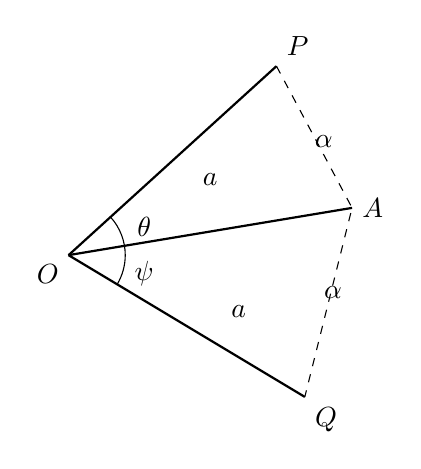
\begin{tikzpicture}[scale=1.2, >=stealth]
  \coordinate (O) at (0,0);
  \coordinate (A) at (3.0, 0.5);
  \coordinate (P) at (2.2, 2.0);
  \coordinate (Q) at (2.5, -1.5);

  \draw[thick] (O) -- (P) node[above right] {$P$};
  \draw[thick] (O) -- (Q) node[below right] {$Q$};
  \draw[thick] (O) -- (A) node[right] {$A$};
  \draw[dashed] (P) -- (A) -- (Q);

  \node[below left] at (O) {$O$};

  \node at (1.5, 0.8) {$a$};
  \node at (1.8, -0.6) {$a$};
  \node at (2.7, 1.2) {$\alpha$};
  \node at (2.8, -0.4) {$\alpha$};

  \draw (0.6,0) arc (0:42:0.6);
  \node at (0.8, 0.3) {$\theta$};

  \draw (0.6,0) arc (0:-31:0.6);
  \node at (0.8, -0.2) {$\psi$};
\end{tikzpicture}
\end{center}

\noindent
正弦定理から
\[
OP = \frac{a \sin\alpha}{\sin(\pi - \theta - \alpha)}, \quad OQ = \frac{a \sin\alpha}{\sin(\pi - \psi - \alpha)}
\]
だから ①から、$OP = OQ$ の時、$\sin(\pi - \theta - \alpha) = \sin(\pi - \psi - \alpha)$ なので
\[
\sin(\theta - \alpha) + \sin(-\psi + \alpha) = 0
\]
\[
-2 \sin\left(\frac{\theta - \psi}{2}\right) \cos\left(\frac{\theta + \psi}{2} - \alpha\right) = 0
\]
$0 < \frac{\theta + \psi}{2} < \frac{\pi}{2}, 0 < \alpha < \pi$ から
\[
\theta = \psi \quad \text{or} \quad \frac{\theta + \psi}{2} = \alpha
\]
$\theta = \psi$ の時 OK、$\frac{\theta + \psi}{2} = \alpha$ の時これを満たす $\alpha$ は2つはないからアウト。

\newpage

\end{document}
